
\chapter{Spring Sampling}
\label{apdx:spring}

\begin{figure}
    \centering
    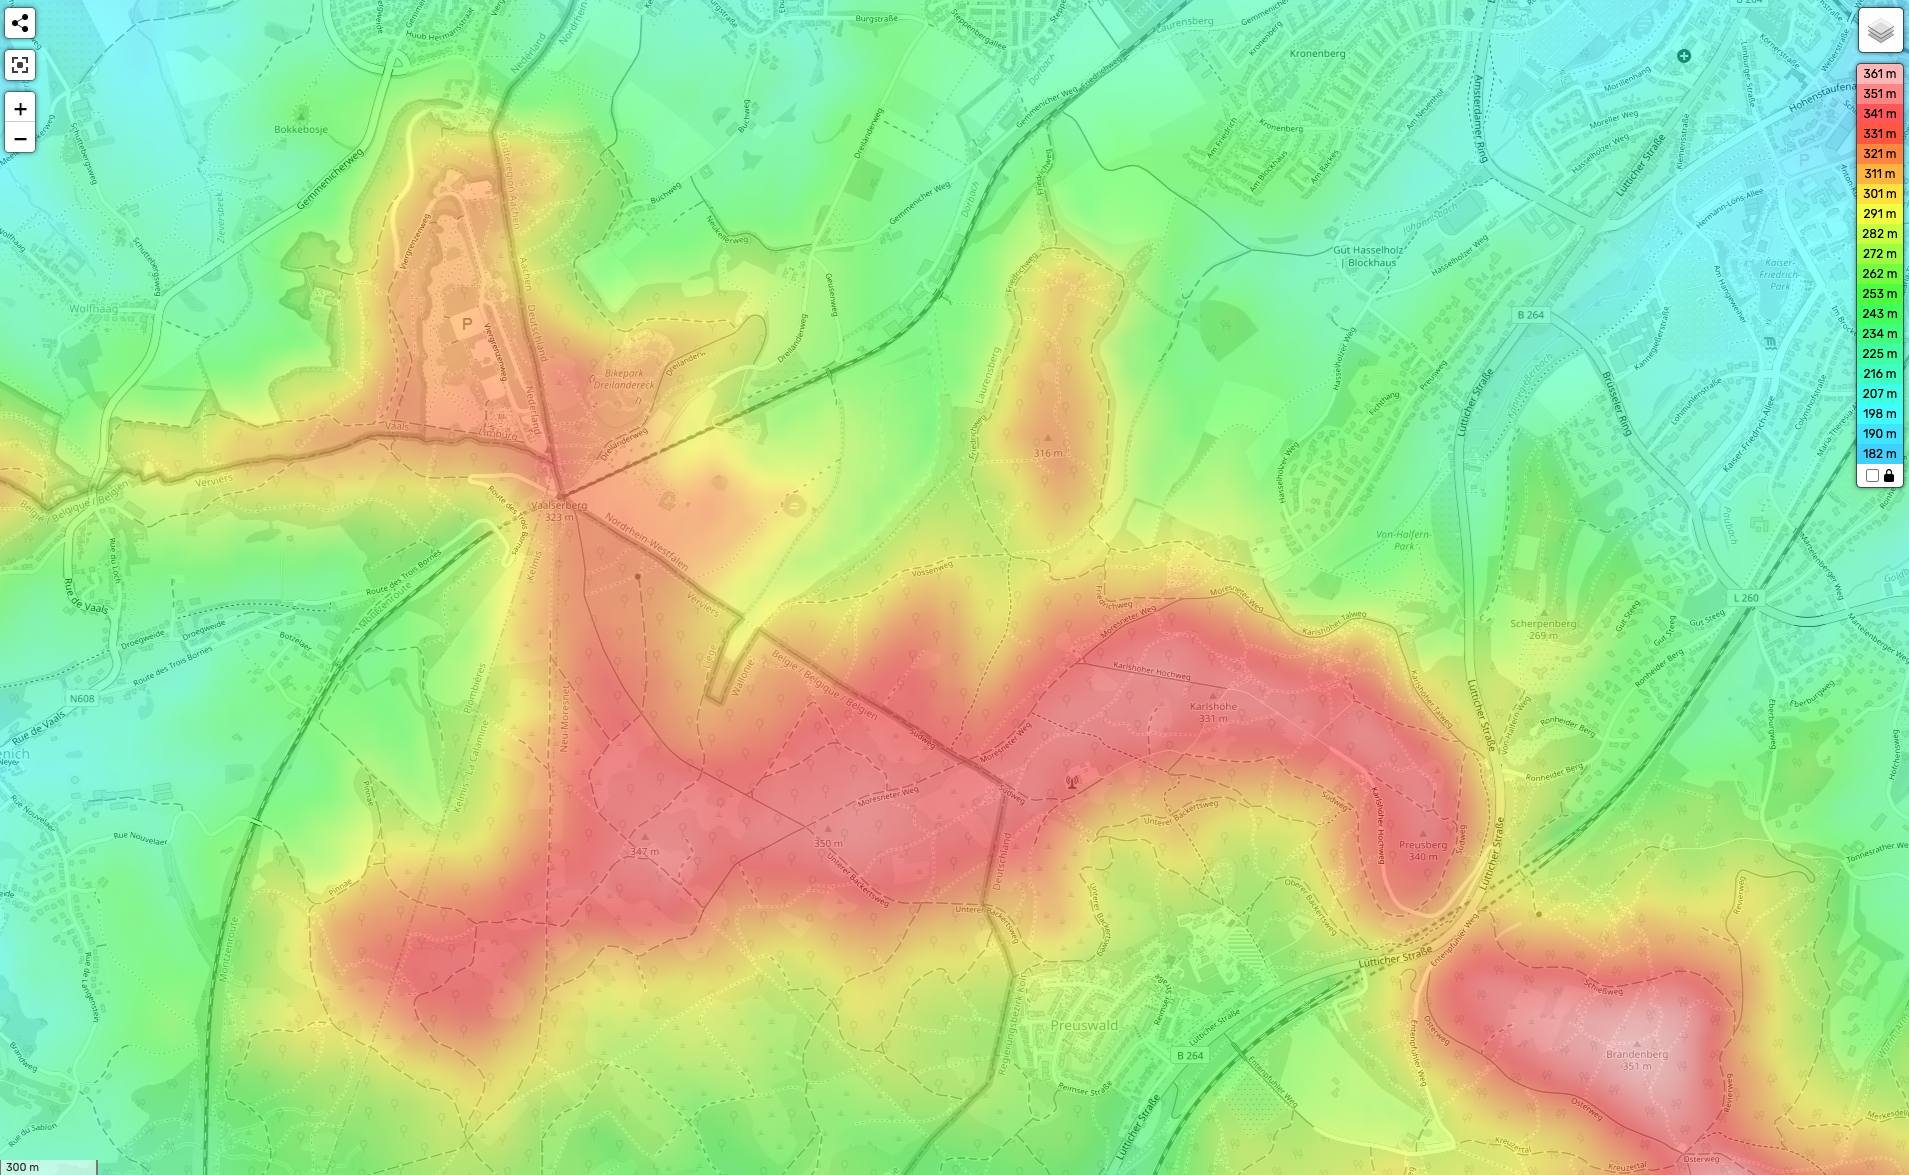
\includegraphics[width=\linewidth]{images/vaalserberg_lost.png}
    \caption{Vaalserberg elevation map}
    \label{fig:vaalserberg-q}
\end{figure}


Consider the search problem displayed on figure \ref{fig:vaalserberg-q}. 
This elevation map of Vaalserberg (the hill that acts as a three-way border between Belgium, the Netherlands and Germany) contains a telecommunications tower. 
Can you find it? Hint: in a hilly terrain, telecommunication towers work better when they are higher up.

If you are anything like me, you would start by looking at the highest points on the map.
If the tower is not there, you would move your gaze (more or less randomly) around the highest parts of the map.
If it's still not found, you would gradually include lower and lower parts of the map into the search space covered by the random walk of your gaze.
At some point, if you still do not see the communications tower, your gaze will be dashing all over the map, including the lowest points.

Let us now formalize this algorithm mathematically.

The height above sea level of a point on this map is a heuristic function that represents the probability $\prob(x)$ of a telecommunications tower being located at point $x$.
We can search the area by sampling points $x \sim \prob(x)$ and checking whether a tower is present at $x$, i.e. whether $\temp(x)=1$.
We can control how much attention we give the high elevation/high likelihood points versus low elevation/low likelihood points with a technique known as \emph{temperature sampling}: define temperature $\temp$ and sample from a modified distribution.

\begin{equation}
\prob_\temp(x) = \frac{\prob(x)^{\frac{1}{\temp}}}{\sum_{x'} p(x')^{\frac{1}{\temp}}}
\end{equation}

When $\temp=0$ we always sample the global maximum: the single likeliest point on the map. 
When $\temp=1$ $\prob_\temp(x)=\prob(x)$.
The higher the temperature $\temp$ the more attention is given to the less likely points in the distribution.

Hence, the technique of looking at the likeliest points first, then gradually including less and less likely ones, corresponds to the following algorithm. At iteration $i$ of our algorithm we sample from the distribution $\prob_\temp(x)$ where temperature is given by

\begin{equation}
\temp = i \Delta \temp
\end{equation}

where $\Delta \temp$ is a hyperparameter that controls the heat input into the system, directly proportional to how impatient the searcher is. So,

\begin{equation}
x \sim \prob_\temp(x) = \frac{\prob(x)^{\frac{1}{i \Delta \temp}}}{\sum_{x'} p(x')^{\frac{1}{i \Delta \temp}}}
\end{equation}

We call this technique \emph{spring sampling}, as it involves gradually, but continuously adding heat to the system until life wakes up therein.

Spring sampling can be used in any \emph{informed search problem} (aka heuristic search problem): find an $x$ such that $\temp(x)=1$ given a heuristic function $\prob(x)$ estimating the probability that $\temp(x)=1$. 
Informed search often comes up in conjunction with machine learning: many machine learning models are probability distributions $\prob(x)$ that estimate how likely some statement is to be true.
For example, a model for ImageNet classification \cite{dengImagenetLargescaleHierarchical2009} us a distribution $p(i,c)$ indicating how likely it is that image $i$ belongs to class $c$.
Likewise, language models are probability distributions $p(w_1,\dots,w_n)$ indicating how likely it is that sentence $w_1,\dots,w_n$ is appears in the training corpus and/or satisfies the human feedback annotator.
A particularly topical (but far from the only) application of spring sampling is thus using a large language model agent to achieve a certain testable goal: sample from the LLM with increasing temperature until the output passes the test.
We use this technique in our program synthesis framework to sample programs that pass a given test suite.
It improves search speed by making sure the likeliest programs are always tested first, but if they do not pass the test, higher temperatures help collect a diverse sample of programs, thus increasing the probability that one of them is correct.

Meanwhile, did you find the tower? Check figure \ref{fig:vaalserberg-a}

\begin{figure}
    \centering
    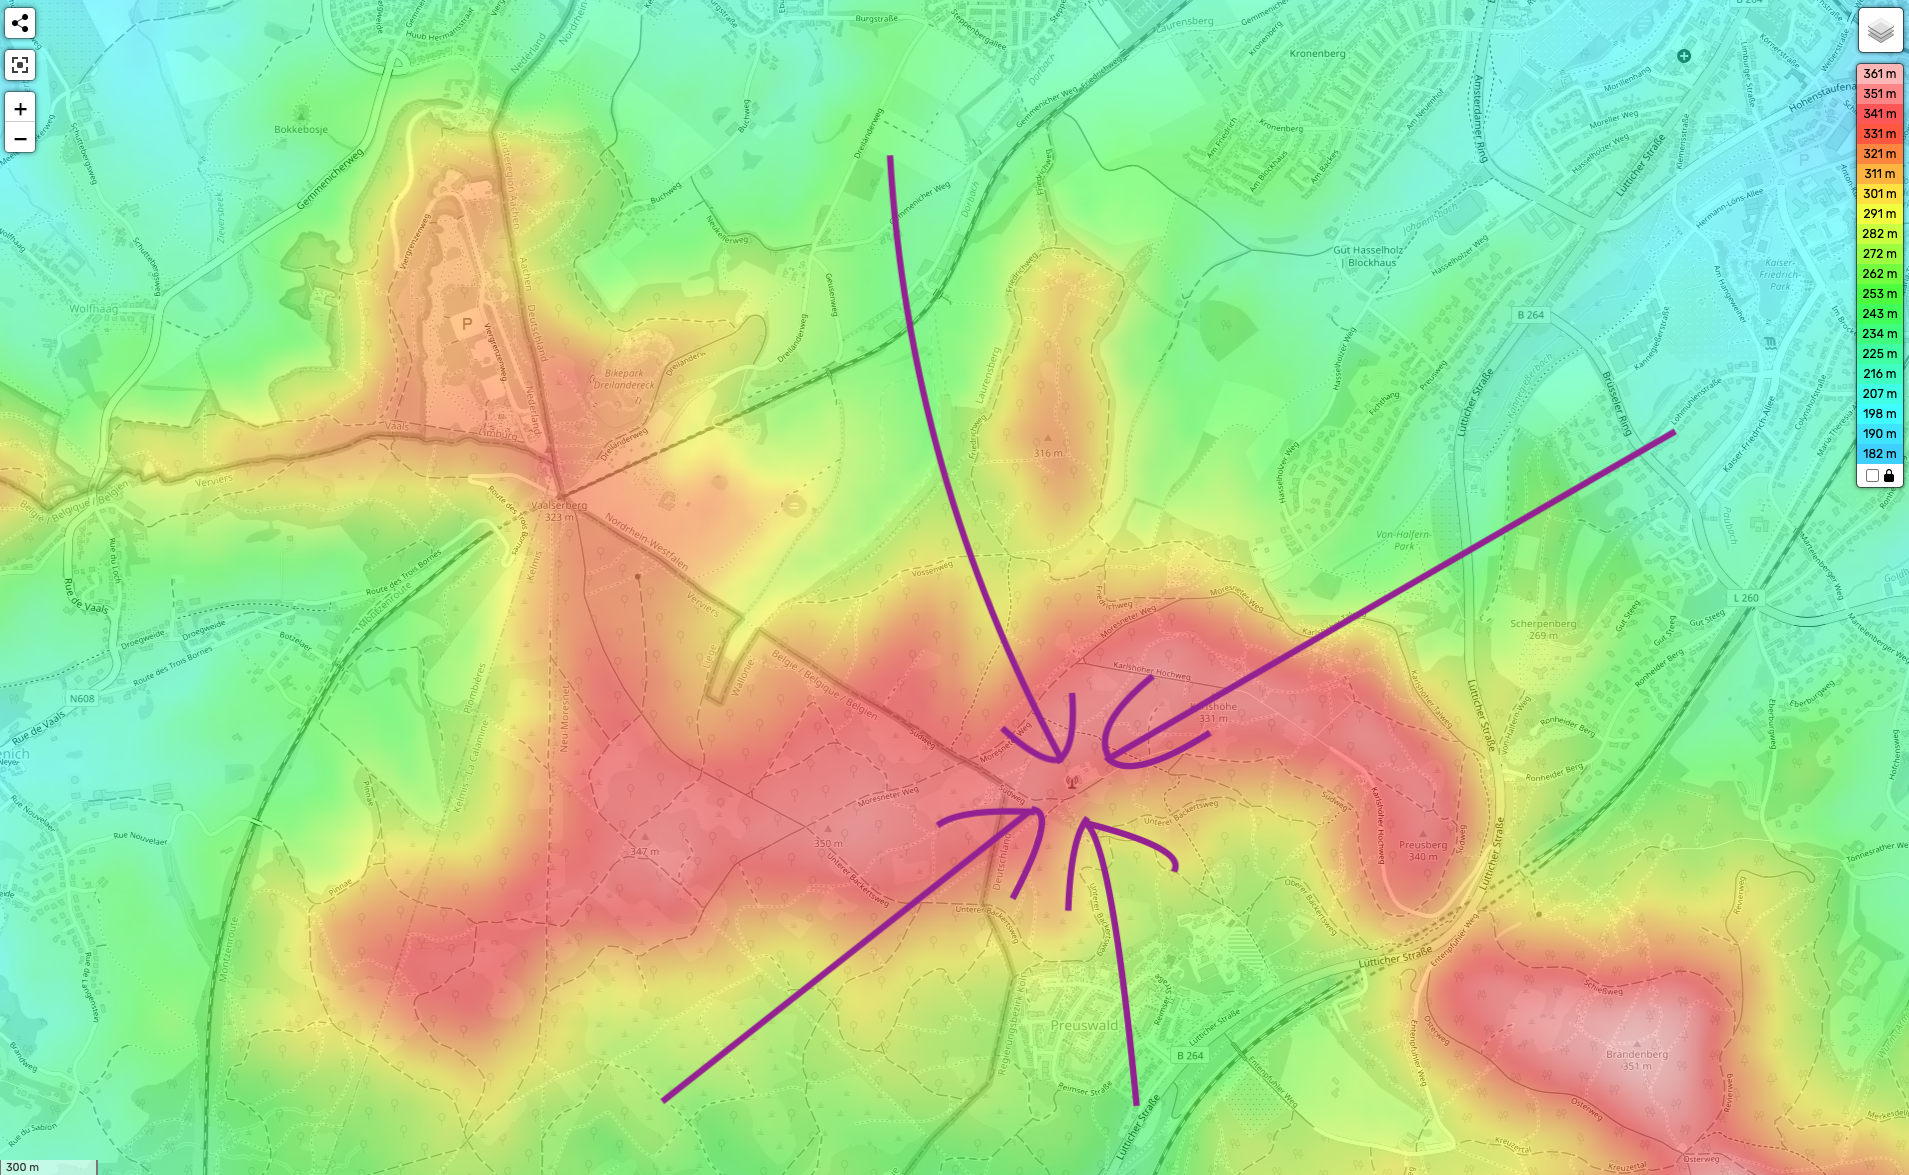
\includegraphics[width=\linewidth]{images/vaalserberg_found.png}
    \caption{Vaalserberg elevation map, tower highlighted}
    \label{fig:vaalserberg-a}
\end{figure}